\subsection*{Acquired local motor content changes the body's subsequent direction}

The preceding cue assays supply either cue-gradient actuation or a common readout of local evidence. A separate experiment asks whether experience can instead establish a bodily movement bias when action and its update remain local. A deformable material body starts with zero two-component motor parameters on a periodic $32\times32$ lattice. Each occupied location perturbs its own motor drive; only actually completed local energy gains and losses provide feedback. The policy receives no global position, field map, hidden outcome sign or reversal clock, and no body-wide action or reward is pooled. Cohesion, pressure, motor axes and the stochastic actuator are preinstalled. Nutritional consequences cover the entire finite substrate, so this is not the sparse recontact problem above. This conservative host has no tissue birth (Supplementary Fig.~\ref{fig:local-motor-content}).

The implementation comparison concerns where the consequence of a local movement is used. In the recipient-credit variant, transported perturbation scores are combined with the paid result at the receiving location. In the source-credit variant, the paid result is returned along the executed transport edges to the location that generated the perturbation; the resulting parameter update is then transported forward with the material. Thus the latter changes both feedback delivery and the site of writing. It is not a clean comparison of optimizers, nor does it identify a unique mediator. The score-based immediate update is a standard simple rule; no new algorithm is inferred from this routing choice.

Two paired seed--field conditions use opposite initial outcome signs. Under source-credit immediate updates, the acquisition-window mean tissue-weighted field scores are $0.72154$ and $0.74061$, with favourable-half mass fractions $0.96399$ and $0.96661$. Both satisfy the original acquisition criterion, whereas the corresponding recipient-immediate cases do not. The two conditions combine different noise/body seeds with opposite fields; they are not a factorial demonstration of generalization across bodies. An exponentially averaged score and an additional occupied-neighbour averaging step fail acquisition in both tested conditions. Their nominal learning rate is shared with the immediate rule, but the normalized exponential average reduces the current perturbation's effective gain. These unoptimized settings do not establish a general inferiority of eligibility traces. The preset eastward control can also obtain positive scores periodically and is retained as an action-capacity control with a directional prior (Supplementary Tables~\ref{tab:motor-phases} and \ref{tab:motor-costs}).

Acquisition is followed by failure to reverse. The actual outcome sign changes at step 321, with paid feedback available immediately. Neither source-immediate path passes the prescribed reversal window: its final-64 mean scores are $-0.18610$ and $-0.01191$, and neither reaches the recorded 32-step recovery criterion during that phase. Only one later no-feedback endpoint passes, giving no complete acquire--reverse--retain life. All six source-credit lives remain viable at mass 24. The failure therefore concerns behavioural revision under the registered opportunities, not material extinction. Continued movement and positive acquisition alone cannot establish adaptation to changed consequences.

We then intervene on the acquired content rather than comparing two already divergent histories. Each complete source-immediate parent at actual step 320 supplies three 128-update futures with payments and new writes disabled. Body, energy, sensory registers, trace and random-generator state are identical within each parent; only the two motor-parameter fields are retained, set to zero or sign-reversed at the branch. Physical dynamics, local exploration and real material transport continue. Along the original learned direction, the two retained branches move $4.3071$ and $4.1842$ lattice units; zeroed branches move $-0.00182$ and $-0.00167$; sign-reversed branches move $-4.4242$ and $-4.3005$. The actual spatial fields and paired displacement distinguish content-dependent action from a difference in initial placement (Supplementary Fig.~\ref{fig:local-motor-content}). Six futures remain two paired parent interventions, not six independent replicates.

The intervention also shows why displacement and useful occupancy must be separated. The zeroed bodies remain in previously acquired favourable locations and pay less for movement: $0.3540$ and $0.3514$, versus $0.4147$ and $0.4128$ with retained parameters. Mean mass in the strongly favourable region is still $22.4977$ and $22.5828$ after zeroing, compared with $23.1507$ and $23.2400$ under retention. These are absolute amounts within bodies of mass 24, not ratios rescued by tiny contact. Their occupancy does not imply learned stopping. Conversely, sign reversal changes the entire subsequent physical future; its effect is not a mediation percentage or a measure of relearning without feedback. Full endpoint energy, occupancy and costs are retained in Supplementary Table~\ref{tab:motor-expression}.

This local, non-renewing host must also be distinguished from the separate regenerative joint-association implementation. That implementation combines a central five-action readout with actual paid births, rule deaths and copying from local pre-write banks. Its four joint lives do not pass the complete behavioural sequence; compact histories can stop at the registered mass floor, while fragmented histories can retain preferences without passing the absolute-contact requirements. The local motor-content intervention here neither supplies that central controller nor tests newborn content. Actual renewal in one implementation and causal motor expression in another do not establish that local learning survives replacement in the same body. The present positive result is narrower and actionable: experience-acquired local content affects whole-body motion, while this acquired-bias implementation fails to revise its direction appropriately after new consequences.

\subsection*{Acquired response gain is sufficient for feedback-triggered turning, but reversal need not require relearning}

The directional-bias result leaves two possibilities: the body may need a new way to update its policy, or it may need to express acquired content conditionally on what it currently senses. We examine that distinction while retaining local execution, actual transport, paid feedback and the no-birth host. In all four new batches, behaviour is scored over the last 64 updates of the prescribed phase using the same field and favourable-mass criteria. These scores describe occupancy. They do not, by themselves, identify how the body arrived there or whether it revised an acquired response.

A linear policy first adds two state-dependent terms to the learned bias, using the previous actual paid-outcome gradient as input. This change does not establish an additional capability. The mass-weighted magnitudes of the two state terms at acquisition are only $0.00246$ and $0.00229$, compared with a bias near $0.656$; the conditional and bias-only paths are nearly coincident. In one condition, both pass the original complete occupancy criterion while continuing mainly in the old direction around the periodic domain. We preserve that passing gate, but do not interpret it as learning to turn (Supplementary Table~\ref{tab:gain-phases}).

An unchanged-relation control from the same complete acquired state explains the ambiguity. Freezing the linear weights leaves the two bodies moving along their original direction whether the payment relation changes or stays unchanged. Their respective 448-update signed displacements are $14.7195/14.5976$ and $14.6945/14.5693$ lattice units under changed/unchanged relations. The nearly same route ends in a favourable region after the change and an unfavourable region without it. At the first continuation update the mean commands, sampled motors and actual transport operators match exactly within all eight pairs. Later payments also change energy and the physical future, so this comparison is not a pure policy-mediation estimate. It nevertheless shows why a favourable endpoint under reversal is insufficient evidence of relearning. The supplied fixed gradient-feedback control actually reverses its command after new feedback, despite failing the earlier prescribed reversal endpoint (Supplementary Table~\ref{tab:gain-relation}).

We next remove the accumulating additive bias and use a standard one-parameter conditional Gaussian policy. The mean command is $\boldsymbol\mu=\kappa\boldsymbol d$, where $\boldsymbol d$ is the unit direction of the last legally observed local paid-outcome gradient and the learned scalar $\kappa$ starts at zero. Local perturbations and their returned consequences update the response gain; transport carries the updated quantity with the material. Gradient direction, Cartesian motor axes and their interpretation as movement remain supplied. This experiment tests acquisition of a usable response strength, not discovery of a sensory direction or a new optimizer (Fig.~\ref{fig:acquired-gain}).

In two new seed--field conditions, both learned-gain lives pass acquisition, reversal and the no-new-feedback aftereffect in the same uninterrupted trajectory. Their phase scores are $0.73116/0.34187/0.57144$ and $0.72261/0.76330/0.78826$. The bias-only and zero-gain controls each have zero complete successes. However, a fixed positive-gain controller, $\kappa=1$, also passes both complete sequences and is a strong alternative: its corresponding scores are $0.97833/0.74831/0.96891$ and $0.97800/0.75103/0.96606$. Thus the new representation enables a conditional capability, but no advantage over the supplied simple direction-following rule is established. This result does not change the earlier immediate-bias experiment's acquisition $2/2$ and reversal $0/2$ outcomes.

The causal role of acquired gain is narrower than the aggregate phase result. From each actual learned body at step 320, we stop only gain writing while retaining real sensing, material transport and physical feedback. Both continuations still pass reversal and aftereffect. The first changed payment arrives at step 321, after that step's action; the updated legal gradient can alter the next command at step 322. Existing gain combined with new sensory evidence is therefore sufficient for the tested change of direction. Successful behaviour after a hidden reversal does not demonstrate that the gain had to be learned again.

Content interventions identify what remains necessary in these two acquired parents. Clearing only $\kappa$ while continuing to freeze its writes makes both reversal and aftereffect fail: their scores are $-0.82935/-0.82263$ and $-0.81331/-0.81299$. Replacing the spatial gain field by its original body-mass-weighted mean succeeds in both parents, with scores $0.57261/0.89549$ and $0.61592/0.89470$, close to the retained/frozen references $0.56962/0.88502$ and $0.61387/0.88362$. The acquired scalar content is usable, whereas its particular heterogeneous distribution is not required in these continuations. These are two matched parents with dependent futures. Erasure changes the drive immediately, and homogenization matches the scalar mean rather than every nonlinear action; neither intervention identifies a unique mediator or a matched-drive effect (Supplementary Table~\ref{tab:gain-parent}).

All 32 recorded paths survive with mass approximately 24, including the failed behavioural conditions and dependent branches. The learned-gain lives end with energies $123.976$ and $133.707$ and spend $2.44816$ and $2.56605$ on movement; the fixed-gain controls end at $144.351$ and $144.347$ while spending $2.81298$ and $2.83660$. Greater movement cost can accompany stronger occupancy and higher energy, so no simultaneous-improvement requirement is imposed. All phase outcomes, payments, basal costs and physical checks remain in Supplementary Tables~\ref{tab:gain-phases}--\ref{tab:gain-material}. During the final 128 updates there are no new payments or new reward-gradient observations: previously lawful records are transported and read. This finite aftereffect does not establish sustained current sensing, general adaptation, or learning maintained through tissue renewal. The latter remains a separate question in the regenerative host.

\begin{figure}[p]
\centering
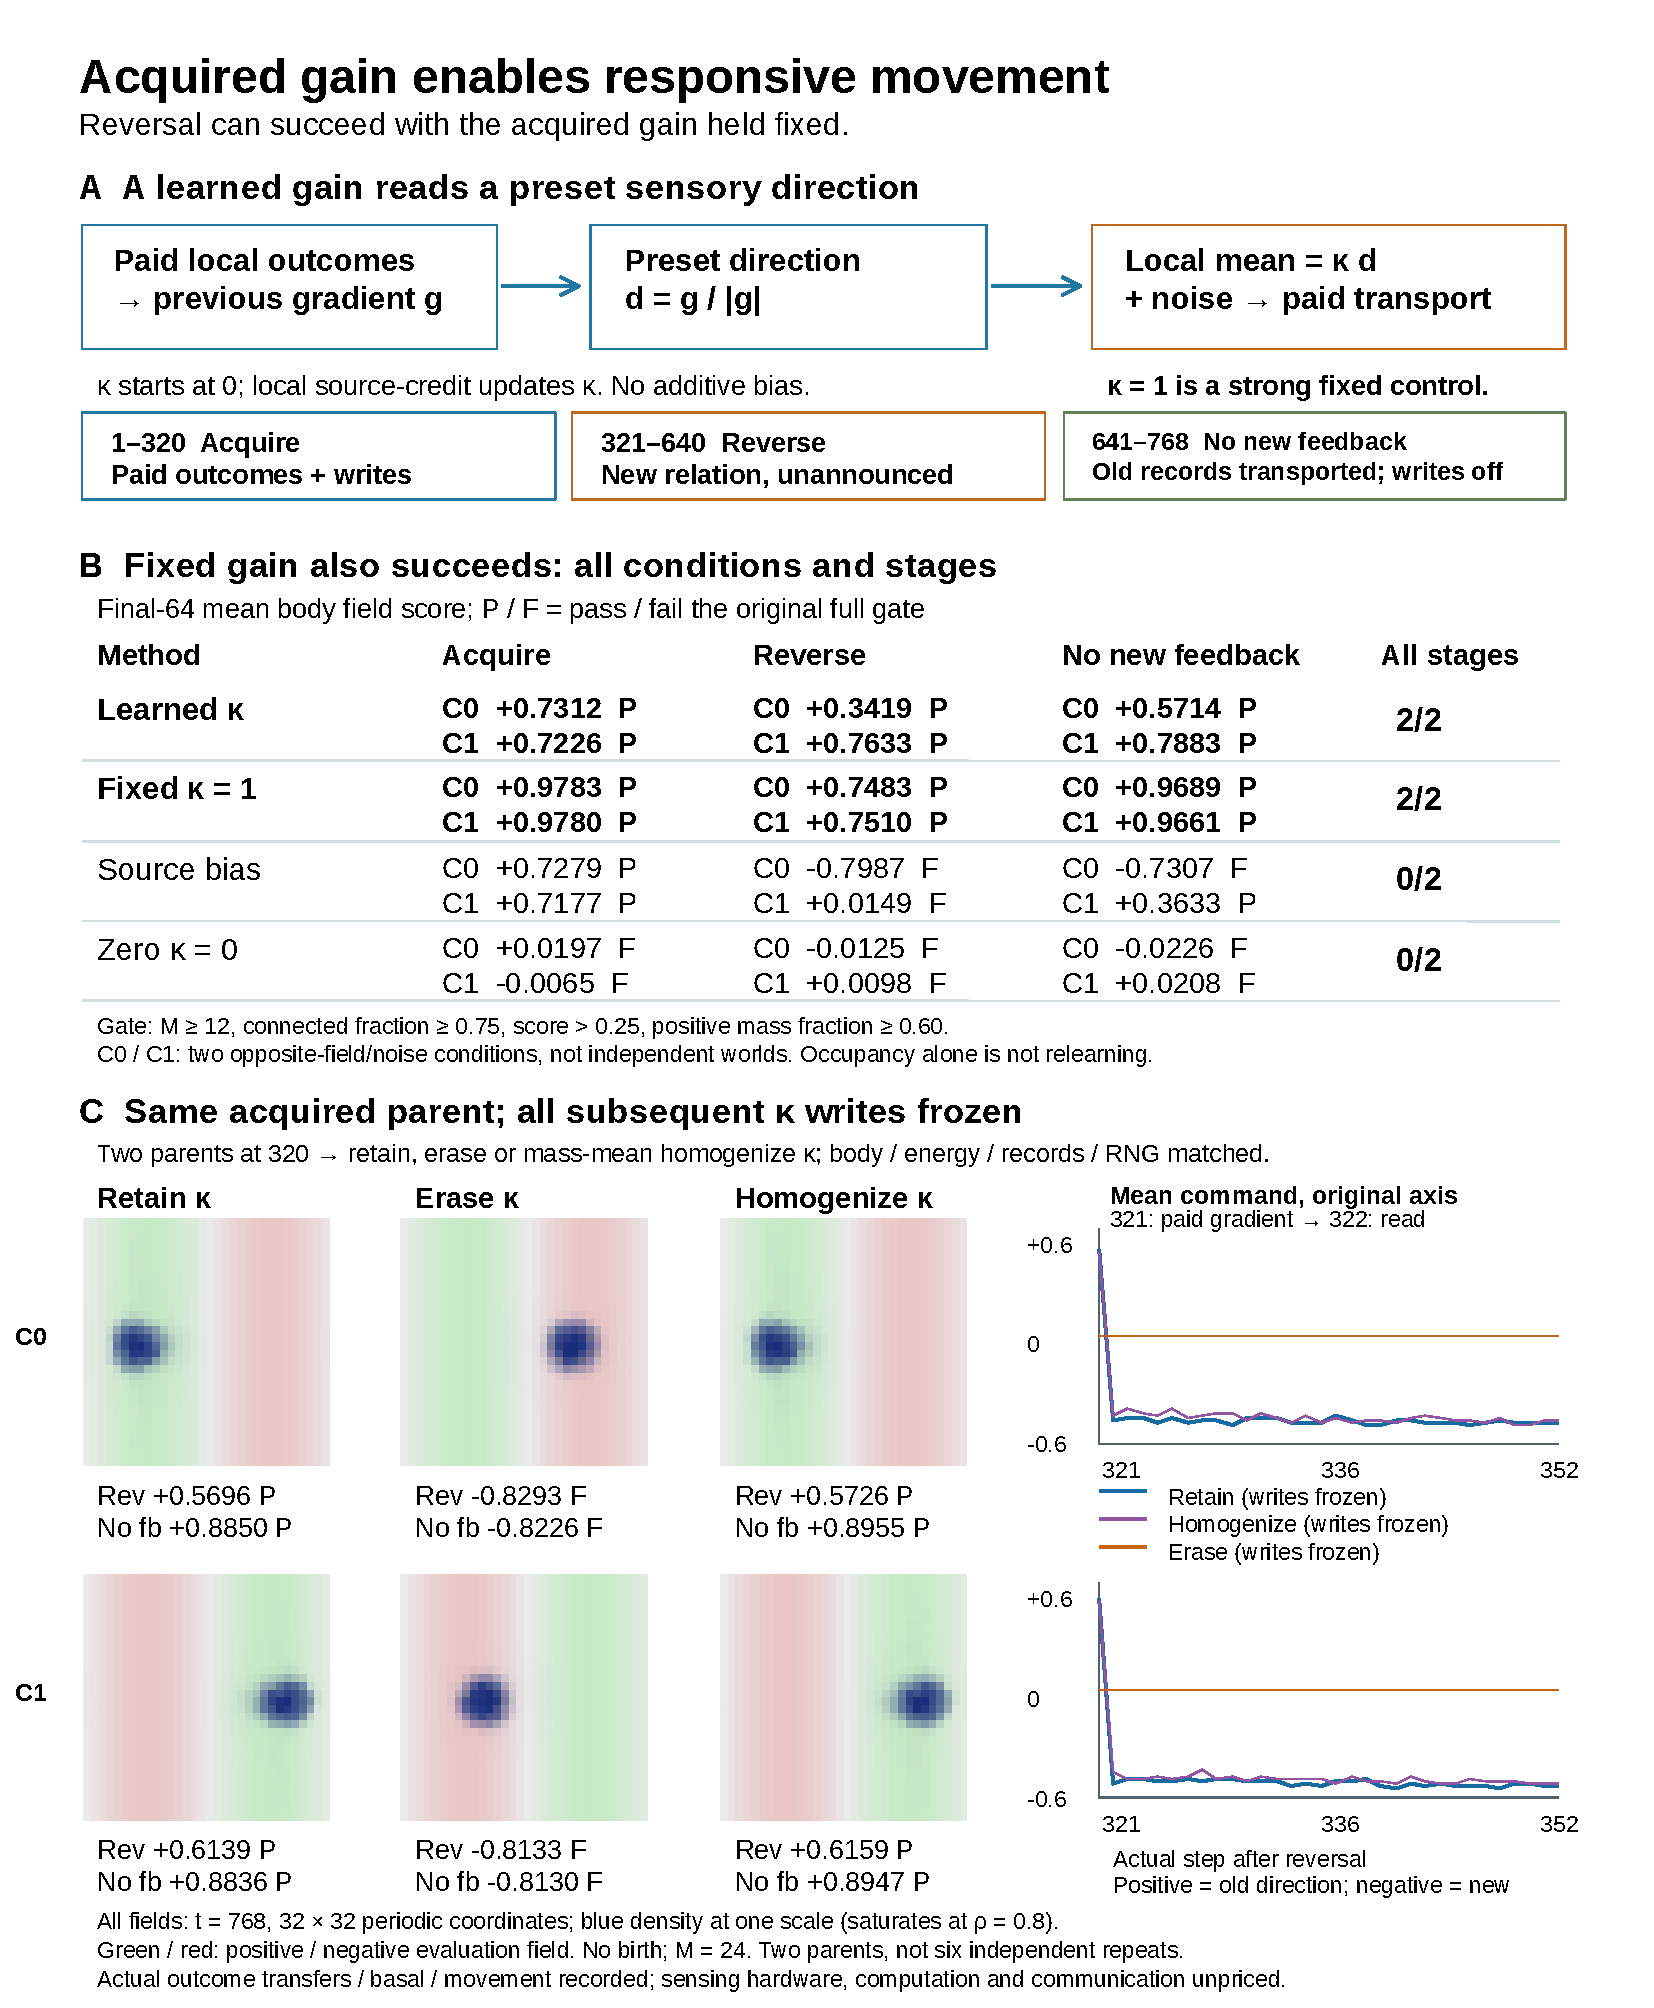
\includegraphics[width=\linewidth,height=0.69\textheight,keepaspectratio]{work/longform_v047/figures/acquired_gain_v0476/acquired_gain.pdf}
\captionsetup{font=footnotesize}
\caption{\textbf{Acquired response gain supports turning without a requirement to relearn the reversal.}
\textbf{a}, A standard local score rule learns an initially zero scalar gain multiplying the direction of a previous actually paid local gradient. Sensory direction and the actuator are supplied. Acquisition and unannounced reversal each last 320 updates; the final 128 add no new payments, observations or writes, while older legal records are transported and read.
\textbf{b}, All four methods and both seed--field conditions retain their final-64 field scores and original composite gates. Learned and fixed positive gain each pass all three phases in both conditions; bias and zero-gain controls do not. Passing the occupancy criterion is not by itself evidence of relearning. Physical costs are reported separately.
\textbf{c}, Two actual acquired parents at 320 supply retained, erased and mass-mean-homogenized gain continuations with gain writing frozen. Retention and homogenization pass both later phases; erasure fails. Curves show the actual mean commands at updates 321--352, not displacement; they change after the new paid observation despite frozen gain. The displayed fields are actual states at update 768 and use original periodic coordinates and a common density scale: blue opacity is $\min(\rho/0.8,1)$, with green/red indicating favourable/unfavourable evaluation fields. Scores under fields describe phase windows, not the displayed snapshot. The six futures are paired interventions from two parents. Homogenization preserves the scalar mean, not each nonlinear action, and global averaging is used only to construct the intervention. All paths remain mass 24 with no tissue birth. Local outcome transfers, basal and movement costs are recorded; computation, communication and sensing hardware have no separate tariff. These results establish a usable acquired response strength, not superiority to fixed positive gain, spatial-pattern necessity, or learning through regeneration.}
\label{fig:acquired-gain}
\end{figure}

